%************************************************
\chapter{Parallelism}\label{ch:Parallelism}
%************************************************
Nowadays, there are more and more cores and computational units in computers and clusters. The problem is that extracting parallelism from a source code is not that easy, so the automatic parallelisation of nowadays languages is a challenge. For example, decide automaticaly to run a code on a GPU or a CPU requires an in-depth knowledge of the code and of the architecture. We will see in this chapter what is parallelism and describe the current architectures.

\section{Definitions}
Parallelism is a kind of computation in which multiples computations are carried out in the same time. The main idea of parallelism is to extract from a big problem multiples smalls problems that can be solved in parallel. 

There are several types of parallelism :
\begin{itemize}
\item Bit-Level parallelism : BLP is based on the size of the processor word size. For instance, to compute an addition of two 32 bits integers, a 16 bits processors will need two cycles whereas a 32 bits processor will only need one.
\item Instruction-Level parallelism : ILP works, as its name suggests, at Instruction level. This means that the dependencies of the code will be analyzed to be able to execute multiples instructions in parallel. Let take an example :
\begin{lstlisting}
S1: a = 2
S2: b = a + 3
S3: c = a*a
\end{lstlisting}
S2 and S3 depends on S1 but S2 and S3 are independant. So it is possible execute simultaneously S2 and S3.

There are multiples optimisations in modern compilers that act at Instruction-Level : Register renaming, Static Expansion etc.
\item Data parallelism : DP is the art of splitting data to multiples computational units, let them compute intermediate results and reconstruct the final results from the intermediate results. Figure~\ref{fig:Data_Parallelism} shows an example of data parallelism to compute a function on an array on two nodes.
\begin{figure}
\centering
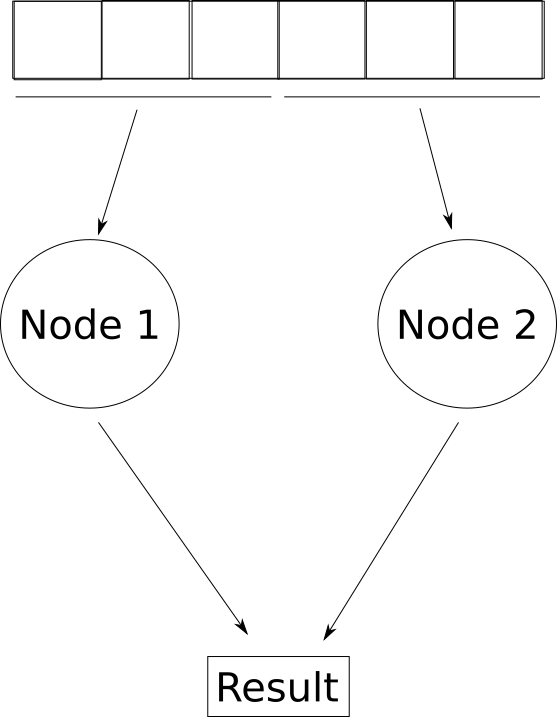
\includegraphics[width=6cm]{gfx/Parallelism/Data_Parallelism.png}
\caption{Splitting of an array to 2 nodes}
\label{fig:Data_Parallelism}
\end{figure}
\item Task parallelism : TP is the art of distributing differents tasks (handle graphical interface, compute price of flight ticket) on multiples computational units. For instance, if you read this document on your computer, there are probably one thread for your favorite pdf reader and one for your system. 
\end{itemize}

Parallelism can be found at two stages :
\begin{itemize}
\item Software : Even if the most common languages were created for non-parallel architectures, more and more library or compilers options are developped to enhance parallelism during compilation/execution. Some implicitly parallel languages exist (\href{https://texasmulticore.com/technology/sequencel-at-a-glance/}{SequenceL} for instance) but are not widely used.
\item Hardware : Some architecture are better for few kind of computation. For example, GPU behave well with array operations. The architecture (memory types and placement, type of nodes and computational units) allows better performance and parallelism  for only a restrict number of cases. Parallelism is the art of building a system that fit to our needs.
\end{itemize}

\section{Architectures}
In this section, we will describe the main architectures that are available to execute programs. The principle, advantages and disavantadges of each will be presented.

\subsection{CPU}
A Central Processing Unit (CPU) is the part of computers that do the computations. This is the most common type of computational units, everyone has one in its machine. The market is flooded  by \href{www.intel.com}{Intel} and \href{www.amd.com}{AMD}. A processor can have one or multiple cores (nowadays 2 to 8), each core is an independant computational unit but the memory is shared between all of them. Figure~\ref{fig:VonNeumann} shows a well known drawing called Von Neumann architecture. On the left, the processor with 4 cores. On the right, the memory. These two components interact together in both direction (CPU to Mem, Mem to CPU).
\begin{figure}
\centering
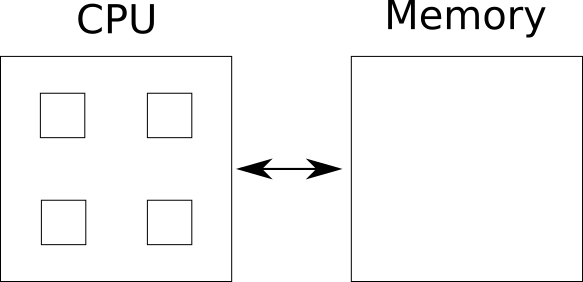
\includegraphics[width=6cm]{gfx/Parallelism/VonNeumann.png}
\caption{Von Neumann architecture}
\label{fig:VonNeumann}
\end{figure}

A CPU executes a flow of instructions according to a fixed pipeline. The most simple pipeline is Instruction Fetch, Instruction Decode, Execute, Write Back.
\begin{itemize}
\item Fetch : The instruction is loaded from the main memory.
\item Decode : The instruction is decoded inside the processor, ie the processor understands what it has to compute.
\item Execute : The computation is done.
\item Write Back : The result is written back in memory.
\end{itemize}

\todo{dessin pipeline}

To enhance the performance of a program, some optimisations can be done at Pipeline-Level. For example, speculative execution allows the processor to load instruction before the end of others running instructions. \todo{faire example de boucle qui charge la dereniere iteration alors qu'il fallait pas}

The advantage of a CPU is that it is possible to design instructions for every specific needs : there are some instructions only used for cryptography in our modern processor. The disavantadge is that the circuit become bigger and bigger and so slower and slower. A CPU follows a single instruction single data  schema : this means that one instruction operate on one data. Performance on vector operations are bad that is why modern processors have Single Instruction Multiple Datas (SIMD) instructions that can perform the same operations on multiple data (doing +2 on all cells of an array for example).

\subsection{GPU}
A \emph{Graphics Processing Unit}, or \emph{GPU}, is a circuit that has been designed to efficiently manipulate images. Every devices that have a screen have a GPU. A GPU contains a lot of simple core that can operates in parallel. At the begining, GPU were designed to rendered images, especially for video games. Today, they are used in others fields like high performance computing. Some GPU does not even have video output : such cards are called accelerators.

At the beginning of computation on GPU, the programers had to convert their problems into a shader version because GPU are only able to make computation on shaders. \todo{lien vers ce qu'est un shader}. Nowadays, some high level framework has been developped to abstract all the shader mechanisms. The most common one is \emph{CUDA} \todo{lien vers cuda} developped by NVIDIA, for NVIDIA cards. The main idea of CUDA is the separation between the Host (the CPU) and the Device (the GPU). The CPU asks to the Device to run a kernel on an array. Then, datas are transfered to the GPU. The GPU operates on the data and finally the results are send back to the CPU. All the memory transferts are very costly but the acceleration provided by the GPU makes the whole process faster. 
\todo{example kernel}

To sum up the advantage of GPU, they can operate way more faster than CPU on array computations. But for that, code should have less dependencies as possible.

\subsection{Others architectures}
ManyCore are processors that contains multiples (10 to 1000) simpler and independant cores. They can be seen as a small cluster inside a chip. This means that programming models like OpenMP or MPI can be used to compiled a code to a ManyCore target. Sunway TaihuLight, a chinese supercomputer is build from 40960 homemade manycores.

Application-Specific Integrated Circuit (ASIC) are processors that are designed for a specific use cases and are not reprogrammable. For instance, if a system need an efficient circuit that compute Fourrier transform, this can be implemented in a ASIC. The advantage is that, due to the fact that the ASIC is designed for a specific use, the performance will be better than with a CPU.

Field-Programmable Gate Array (FPGA) are between ASIC and CPU. FPGA are circuit that can be reconfigured multiples times but one configured can only do one things. For instance, some prototypes chips have a CPU and a FPGA so that if the compiler detects a piece of code that are run multiple time, it will configure the FPGA to do this operation and let the CPU ask the FPGA each time it needs the value.  

\section{Dependencies analysis}
Dependencies analysis is a way to get constraints between statements in a program. There are two types of dependencies :
\begin{itemize}
\item \emph{Control dependencies} happen when execution of a statement depends on the result of a previous instruction. 
\begin{lstlisting}
S1: if (N<10)
S2:     A[i] = 0;
\end{lstlisting}

For this example, we say that S2 is control-dependent on S1.


\item \emph{Data dependencies} happen when two different statement access the same ressource.
\end{itemize}

Data dependencies can appears in four different manner :
\begin{itemize}
\item \emph{Flow Dependences}, or \emph{Read After Write} happen when an instruction S2 reads the data modified by an instruction S1 that preceeds S2. 
\begin{lstlisting}
S1: x = 10
S2: print(x)
\end{lstlisting}
In this example, it is impossible to reorder or parallelize the execution.

\item \emph{Antidependencies}, or \emph{Write After Read} happen when an instruction S2 writes the data read by an instruction S1 that preceeds S2.
\begin{lstlisting}
S1: print(x)
S2: x = 10
\end{lstlisting}
In this example, it is impossible to reorder or parallelize the execution.

\item \emph{Output Dependences}, or \emph{write After Write} happen when an instruction S2 writes the data modified by an instruction S1 that preceeds S2.
\begin{lstlisting}
S1: x = 10
S2: x = 20
\end{lstlisting}
In this example, it is impossible to reorder or parallelize the execution.

\item \emph{Input Dependences}, or \emph{Read After Read} happen when an instruction S2 reads the data read by an instruction S1 that preceeds S2. 
\begin{lstlisting}
S1: print(x)
S2: y = x
\end{lstlisting}
In this example, it is possible to reorder or parallelize the execution.
\end{itemize}

\emph{WAR} and \emph{WAW} are called \emph{name dependencies} and can be remove by variables renaming or static expansion. Let take an example :
\begin{lstlisting}
S1: B = 2
S2: A = B + 2
S3: B = 3
\end{lstlisting}

There are a RAW dependency between S2 and S1, a WAR between S3 and S2 and a WAW between S3 and S1. It is possible to remove WAR and WAW by renaming variables :
\begin{lstlisting}
S1: B2 = 2
S2: A = B2 + 2
S3: B = 3
\end{lstlisting}
Now, we only have one RAW dependency between S2 and S1 and we will never be able to remove this one because this dependency represents the natural flow of the program.
